\chapter{Arhitektura i dizajn sustava}

	\begin{itemize}
		\item \textbf{Proces odabira arhitekture}

Razmatrajući cilj projektnog zadatka, koji je izrada web aplikacije koja olakšava pronalaženje i organizaciju plesnih tečajeva i plesnjaka, specifikacijom svih dionika i njihovih mogućnosti prilikom korištenja aplikacije te definiranjem funkcionalnih zahtjeva zaključili smo da naša aplikacija mora imati tri osnovne razine – \underbar{razinu klijenta, razinu web-aplikacije te razinu baze podataka.} Također, prateća tri sloja koja odgovaraju navedenoj podjeli – \underbar{sloj korisničkog}
\underbar{sučelja, sloj aplikacijske logike te sloj pristupa podacima.} 

Nadalje, slijedeći principe dobrog oblikovanja, kako bi povećali koheziju i smanjili nepotrebne međuovisnosti, kod koji obavlja pojedinu operaciju vezanu uz određeni entitet je grupiran, dok se sve ostalo što nije izravno vezano uz tu funkcionalnost stavlja izvan te operacije. 

Razine također trebaju formirati hijerarhiju, tako da su svi resursi za pristup skupu povezanih usluga na jednom mjestu, čime se omogućuje da viša razina može putem programskog sučelja pristupiti nižoj. 

Također, kako bi si olakšali snalaženje cilj je grupirati sve dijelove programa koji pristupaju ili mijenjaju određene podatke te grupirati procedure koje se izvode slijedno i izmjenjuju podatke. Pomoćne programe primjenjive na više različitih grupa, koji se logički ne mogu smjestiti u ostale grupe odvajamo u grupu pomoćnih programa (utils/shared/common).

Ovisnosti između pojedinih modula želimo smanjiti kako nam neke jednostavnije izmjene ne bi zahtijevale promjene na velikom broju ostalih modula te želimo da nam se jasno vidi povezanost određenih entiteta i njihovih odgovarajućih sučelja. 

U aplikaciji također želimo ostvariti povećanje ponovne uporabivosti što ćemo postići korištenjem programskih knjižnica i radnih okvira. 

Nakon svih razmatranja odabrali smo višeslojnu arhitekturu temeljenu na odnosu klijent-poslužitelj, najsličniju MVC stilu arhitekture.


		\item  \textbf{Višeslojna arhitektura}

Karakteristika klijent-poslužitelj opisuje odnos programa koji surađuju u aplikaciji. Ovaj model arhitekture uključuje razmatranje funkcioniranja klijenta i poslužitelja prije, tijekom i po završetku zajedničke komunikacije.


Aplikacija ima tri osnovna sloja:

1.\textit{Klijentsku komponentu} – sloj s korisničkim sučeljem

2.\textit{Poslužiteljsku komponentu} – sloj aplikacijske logike s implementacijom poslovnih procesa i izračuna

3.\textit{Bazu podataka} – podatkovni sloj za pohranu podataka


\underbar{Klijentska komponenta} predstavljena je web preglednikom, programom koji klijentu omogućuje pregled web-stranica i multimedijskih sadržaja vezanih uz te stranice odnosno ima mogućnost pristupa informacijama i zahtijevanja usluga poslužitelja. Web preglednik je prevoditelj koji web stranicu pisanu u kodu interpretira i prikazuje u klijentu razumljivom obliku. Koristeći web preglednik klijent šalje zahtjeve web poslužitelju.

\underbar{Poslužiteljska komponenta} predstavlja web poslužitelj, program čija je osnovni zadatak pohrana, obrada i dostava web stranica klijentu te nam ona predstavlja centar za razmjenu informacija i pružanje usluga. Komunikacija se odvija na aplikacijskoj razini OSI modela koristeći HTTP protokol prijenosa informacija na webu temeljen na izmjeni poruka zahtjev-odgovor. Sam poslužitelj pokreće web aplikaciju i prosljeđuje joj klijentske zahtjeve. 

Web aplikacija obrađuje klijentske zahtjeve pri čemu prema potrebi pristupa bazi podataka te preko poslužitelja, klijentu vraća odgovor vidljiv u web pregledniku.

Prednosti odabrane arhitekture su te što se slojevi mogu oblikovati odvojeno te sve komponente mogu biti jednostavnije i razumljivije, ostvaruje se podjela brige(separation of concerns) time što svaki sloj brine o svojoj funkcionalnosti i ne miješa se u brige nekog drugog sloja, a njihova međuovisnost ostvaruje se komunikacijom putem sučelja čija se implementacija može prilagoditi u određenom sloju.

Za izradu aplikacije kao radni okvir na klijentskoj strani odabrali smo Vue.js zasnovan na JavaScriptu koji pruža učinkoviti razvoj klijentskog sučelja koristeći već dostupne web komponente. 

Za radni okvir na poslužiteljskoj strani odabrali smo radni okvir Node.js Express koji pruža funkcionalnosti posredniče arhitekture (middleware) i usmjeravanja te Sequlize koji apstrahira pristup bazi podataka i omogućuje jednostavnije kreiranje upita bez obzira koja se baza koristi.

Članovi tima kod pišu u razvojnom okruženju Visual Studio Code, no to razvojno okruženje nije nužno i može se koristiti bilo kojim drugim uređivačem teksta. Jednostavno pokretanje, konfiguraciju i puštanje u pogon te neovisnost o računalu na kojem se kod izvršava omogućava korištenje platforme Docker. Kroz 3 Docker kontejnera pokriveni su svi ključni djelovi/slojevi aplikacije - klijent, poslužitelj i baza podataka te su osigurane točne verzije svih vanjskih biblioteka i alata.

%unos slike
		\begin{figure}[H]
			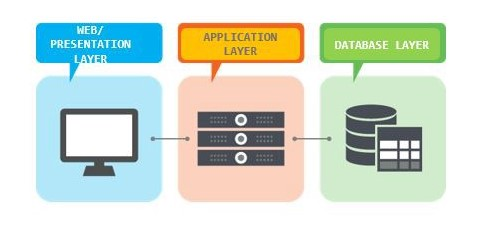
\includegraphics[scale=0.6]{slike/slojevi.jpeg} %veličina slike u odnosu na originalnu datoteku i pozicija slike
			\centering
			\caption{Slojevi arhitehkture}
			\label{fig:sa}
		\end{figure}


		\item \textbf{MVC stil arhitekture}

Arhitektura je  detaljnije razrađena najsličnija stilu arhitekture MVC (Model-View-Controller).

Osnovna karakteristika ovog stila je nezavisan razvoj pojedinih dijelova aplikacije što omogućuje jednostavnije testiranje i razvijanje dijelova sustava te njihove dorade. Korisničko sučelje je odvojeno od ostatka sustava,  a kohezija elemenata se postiže kroz tri sloja, jednog sloja na klijentskoj strani - pogled (View) te dva na poslužiteljskoj strani – nadglednik (Controller) i model (Model).

1.\textit{Model} – predstavlja glavnu komponentu sustava koja sadrži dinamičke strukture podataka odnosno razrede koji opisuju domenu primjene te sadrže pravila i aplikacijsku logiku. Blisko je povezan s bazom podataka aplikacije.

2.\textit{Pogled (View)} – komponenta koja sadrži niz drugih komponente koje služe za prikaz podataka modela i interakciju s korisnikom kroz grafičko sučelje.

3.\textit{Nadglednik (Controller)}  – komponenta koja upravljaja korisničkim zahtjevima prema modelu i odgovorima modela natrag prema pogledima. Omogućuje poveznicu korisničke strane s poslužiteljskom.

%unos slike
		\begin{figure}[H]
			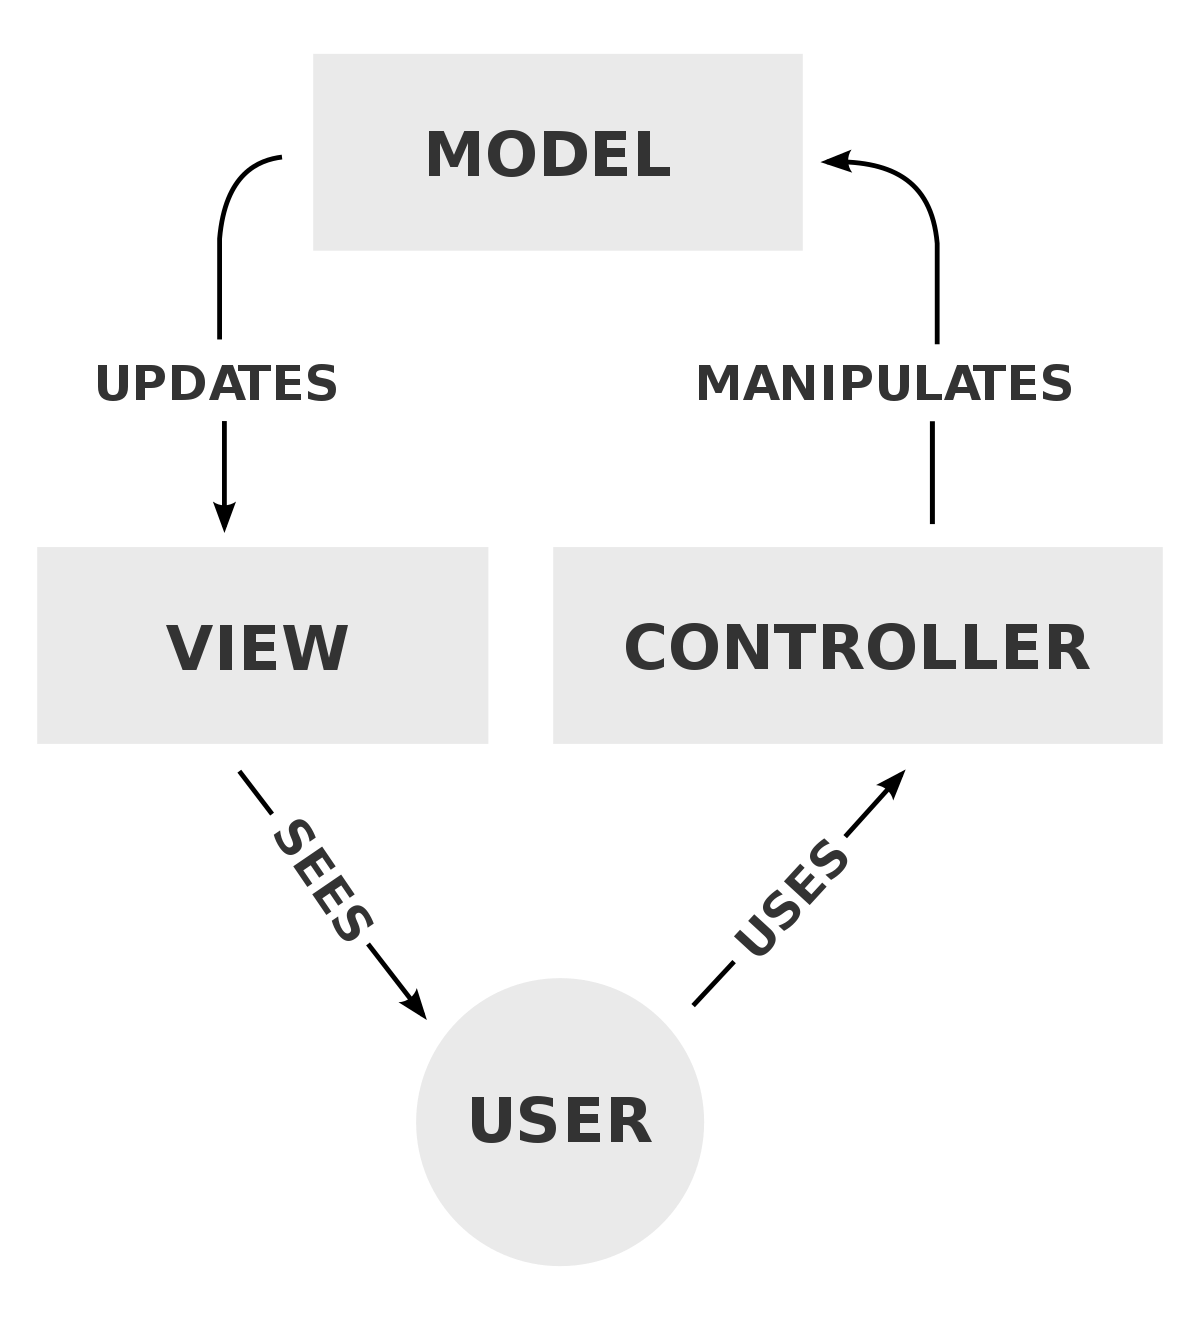
\includegraphics[scale=0.1]{slike/mvc.PNG} %veličina slike u odnosu na originalnu datoteku i pozicija slike
			\centering
			\caption{MVC stil arhitekture}
			\label{fig:mvc}
		\end{figure}
	

	\end{itemize}


		
		\section{Baza podataka}

		Za potrebe našeg sustava koristit ćemo relacijsku bazu podataka koja je jednostavna za modeliranje naših potreba - upravljanje podacima o klubovima koji organiziraju određene događaje i korisnicima koji ih pohađaju. Sastavni elementi baze su relacije, odnosno tablice koje sadrže svoje atribute. Zadaća baze podataka je jednostavna pohrana,umetanje, izmjena i dohvat podataka za daljnju obradu. Baza podataka ove aplikacije sastoji se od sljedećih tablica:

			\begin{packed_item}
			\item  User
			\item  Club
			\item  Course
			\item  UserCourse
			\item  TrainerAplication
			\item  Event
			\item  Dance
			\item  Location
			\item  EventDance
			\item  Lesson
			\end{packed_item}

			\subsection{Opis tablica}
				\noindent\textbf{User} Ovaj entitet opisuje korisnike i sadrži sve informacije o njima. Povezan je sa vezom \textit{One-to-Many} sa TrainerAplication preko \textit{trainerId}, \textit{One-to-Many} sa UserCourse preko \textit{userId} i \textit{One-to-Many} sa Club preko \textit{ownerId}.
				\begin{longtblr}[
					label=none,
					entry=none
					]{
						width = \textwidth,
						colspec={|X[6,l]|X[6, l]|X[20, l]|}, 
						rowhead = 1,
					} %definicija širine tablice, širine stupaca, poravnanje i broja redaka naslova tablice
					\hline \multicolumn{3}{|c|}{\textbf{User}}	    \\ \hline[3pt]
					\SetCell{LightGreen} id & int	& jedinstveni identifikator korisnika \\ \hline
					username & varchar & jedinstveno korisničko ime korisnika\\ \hline 
					firstName & varchar & ime korisnika \\ \hline 
					lastName & varchar & prezime korisnika \\ \hline 
					password & varchar & zaporka za prijavu korisnika \\ \hline 
					gender & enum & spol korisnika \\ \hline 
					dateOfBirth & date & datum rođenja korisnika \\ \hline 
					phone & varchar & jedinstveni kontakt broj korisnika \\ \hline 
					email & varchar & jedinstvena email adresa korisnika \\ \hline 
					role & enum & uloga korisnika \\ \hline
					experienceDescription & varchar & opis korisnikovog iskustva u različitim plesovima \\ \hline 
					image & varchar & fotografija korisnika \\ \hline 
					refreshToken & varchar & korisnikov refresh token \\ \hline 
				\end{longtblr}

				\noindent\textbf{Club} Ovaj entitet opisuje klubove i sadrži sve informacije o njima. Povezan je sa vezom \textit{One-to-Many} sa TrainerApplocation preko \textit{id}, \textit{One-to-Many} sa Event preko \textit{id}, {One-to-Many} sa Course preko \textit{id}, \textit{Many-to-One} sa User preko \textit{ownerId}, \textit{Many-to-One} sa Location preko \textit{locationId}.
				\begin{longtblr}[
					label=none,
					entry=none
					]{
						width = \textwidth,
						colspec={|X[6,l]|X[6, l]|X[20, l]|}, 
						rowhead = 1,
					} %definicija širine tablice, širine stupaca, poravnanje i broja redaka naslova tablice
					\hline \multicolumn{3}{|c|}{\textbf{Club}}	 \\ \hline[3pt]
					\SetCell{LightGreen} id & int & jedinstveni identifikator treninga \\ \hline
					\SetCell{LightBlue} ownerId & int & identifikator korsnika [ref: $>$ korisnik.id]\\ \hline 
					name & varchar & ime kluba \\ \hline 
					phone & varchar & kontakt broj kluba \\ \hline 
					email & varchar & kontakt mail kluba \\ \hline 
					description & varchar & opis kluba \\ \hline 
					approvalStatus & enum & status odobrenja kluba\\ \hline 
					locationId & int & identifikator lokacije\\ \hline 
				\end{longtblr}

				\noindent\textbf{Course} Ovaj entitet opisuje tečajeve i sadrži sve informacije o njima. Povezan je sa vezom \textit{Many-to-One} sa User preko \textit{trainerId},  {Many-to-One} sa Club preko \textit{clubId}, {Many-to-One} sa Location preko \textit{locationId}, {Many-to-One} sa Dance preko \textit{danceId}, \textit{One-to-Many} sa UserCourse preko \textit{courseId} i \textit{One-to-Many} sa Lesson preko \textit{id}.
				\begin{longtblr}[
					label=none,
					entry=none
					]{
						width = \textwidth,
						colspec={|X[6,l]|X[6, l]|X[20, l]|}, 
						rowhead = 1,
					} %definicija širine tablice, širine stupaca, poravnanje i broja redaka naslova tablice
					\hline \multicolumn{3}{|c|}{\textbf{Course}}	 \\ \hline[3pt]
					\SetCell{LightGreen} id & int	&  	jedinstveni identifikator tečaja\\ \hline
					\SetCell{LightBlue} locationId	& int & identifikator lokacije [ref: $>$ Lokacija.id]\\ \hline 
					\SetCell{LightBlue} trainerId	& int & identifikator klijenta(trenera) [ref: $>$ Korisnik.id]\\ \hline 		
					name	& varchar &   ime tečaja	\\ \hline 
					description & varchar & opis tečaja  \\ \hline 
					image	& varchar &   url slike za opis tečaja	\\ \hline 
					capacity & int &  kapacitet polaznika \\ \hline 
					minAge	& int &   ograničenje za minimalni broj godina polaznika	\\ \hline 
					maxAge & int &  ograničenje za maksimalni broj godina \\ \hline 
					gender & enum &  ograničenje za spol polaznika 	\\ \hline
					applicationDeadline & datetime & datum za krajnji rok prijave  \\ \hline 
  					maxApplicants & int &  maksimalan broj polaznika \\ \hline 
  					additionalRules & varchar & dodatne informacije i pravila za tečaj  \\ \hline 
  					\SetCell{LightBlue} clubId & int  &  identifikator kluba koji organizira tečaj [ref: $>$ Klub.id]\\ \hline 
  					\SetCell{LightBlue} danceId & int  &   identifikator plesa koji će se plesati na tečaju [ref: $>$ Ples.id]\\ \hline 
					
				\end{longtblr}
				
				\noindent\textbf{UserCourse} Ovaj entitet opisuje korisnike tečaja i sadrži sve potrebne informacije i reference o njima. Povezan je sa vezom \textit{Many-to-One} sa User preko \textit{userId} i \textit{Many-to-One} sa Course preko \textit{courseId}.
				\begin{longtblr}[
					label=none,
					entry=none
					]{
						width = \textwidth,
						colspec={|X[6,l]|X[6, l]|X[20, l]|}, 
						rowhead = 1,
					} %definicija širine tablice, širine stupaca, poravnanje i broja redaka naslova tablice
					\hline \multicolumn{3}{|c|}{\textbf{UserCourse}}	 \\ \hline[3pt]
					\SetCell{LightGreen} id & int	& jedinstveni identifikator  \\ \hline
					\SetCell{LightBlue} userId	& int & identifikator korisnika [ref: $>$ Korisnik.id]\\ \hline 
					\SetCell{LightBlue} courseId	& int & identifikator tečaja[ref: $>$ Tecaj.id]\\ \hline 
					status & enum & status je li korisnik primljen na tečaj \\ \hline 
				\end{longtblr}

				\noindent\textbf{TrainerApplication} Ovaj entitet opisuje korisnike koji su se prijavili za trenera i sadrži potrebne informacije o njima. Povezan je sa vezom \textit{Many-to-One} sa User preko \textit{trainerId} i  \textit{Many-to-One} sa Club preko \textit{clubId}.
				\begin{longtblr}[
					label=none,
					entry=none
					]{
						width = \textwidth,
						colspec={|X[6,l]|X[6, l]|X[20, l]|}, 
						rowhead = 1,
					} %definicija širine tablice, širine stupaca, poravnanje i broja redaka naslova tablice
					\hline \multicolumn{3}{|c|}{\textbf{TrainerApplication}}	 \\ \hline[3pt]
					\SetCell{LightGreen} id & int	& jedinstveni identifikator trenera \\ \hline
					\SetCell{LightBlue} trainerId	& int & identifikator korisnika [ref: $>$ Korisnik.id]\\ \hline 
					\SetCell{LightBlue} clubId & int & identifikator kluba [ref: $>$ Klub.id] \\ \hline 
					motivationLetter & varchar & motivacijsko pismo ___ \\ \hline 
					certificate & varchar & položeni certifikat za trenera \\ \hline 
					status & enum & status odobrenja trenera \\ \hline 
				\end{longtblr}

				\noindent\textbf{Event} Ovaj entitet opisuje plesnjake i sadrži sve informacije o njima. Povezan je sa vezom \textit{Many-to-One} sa Location preko \textit{locationId}, \textit{Many-to-One} sa Club preko \textit{clubId} i \textit{One-to-Many} sa EventDance preko \textit{id}.
				\begin{longtblr}[
					label=none,
					entry=none
					]{
						width = \textwidth,
						colspec={|X[6,l]|X[6, l]|X[20, l]|}, 
						rowhead = 1,
					} %definicija širine tablice, širine stupaca, poravnanje i broja redaka naslova tablice
					\hline \multicolumn{3}{|c|}{\textbf{Event}}	 \\ \hline[3pt]
					\SetCell{LightGreen} id & int	& jedinstveni identifikator plesnjaka \\ \hline
					\SetCell{LightBlue} locationId	& int & identifikator lokacije[ref: $>$ Lokacija.id]\\ \hline 
					\SetCell{LightBlue} clubId	& int & identifikator kluba[ref: $>$ Klub.id]\\ \hline 
					name & varchar & naziv plesnjaka \\ \hline 
					description & varchar & opis plesnjaka \\ \hline 
					image & varchar & slika plesnjaka \\ \hline 
				\end{longtblr}

				\noindent\textbf{Location} Ovaj entitet opisuje lokaciju sa imenom i koordinatama pomoću kojih se prikazuje na karti. Povezan je sa vezom  \textit{One-to-Many} sa Event preko \textit{locationId}, \textit{One-to-Many} sa Course preko \textit{courseId} i \textit{One-to-Many} sa Club preko \textit{locationId}.
				\begin{longtblr}[
					label=none,
					entry=none
					]{
						width = \textwidth,
						colspec={|X[6,l]|X[6, l]|X[20, l]|}, 
						rowhead = 1,
					} %definicija širine tablice, širine stupaca, poravnanje i broja redaka naslova tablice
					\hline \multicolumn{3}{|c|}{\textbf{Location}}	 \\ \hline[3pt]
					\SetCell{LightGreen} id & int	&  jedinstveni	identifikator lokacije 	\\ \hline
					name	 & varchar &   ime lokacije	\\ \hline 
					coordinates & varchar & geografska širina i dužina lokacije na karti  \\ \hline 
					
				\end{longtblr}
				
  				\noindent\textbf{EventDance} Ovaj entitet opisuje identifikatore plesnjaka i identifikatore plesova koji se na njima plešu. Povezan je sa vezom  \textit{Many-to-One} sa Event preko \textit{eventId} i \textit{Many-to-One} sa Dance preko \textit{danceId}.
				\begin{longtblr}[
					label=none,
					entry=none
					]{
						width = \textwidth,
						colspec={|X[6,l]|X[6, l]|X[20, l]|}, 
						rowhead = 1,
					} %definicija širine tablice, širine stupaca, poravnanje i broja redaka naslova tablice
					\hline \multicolumn{3}{|c|}{\textbf{EventDance}}	 \\ \hline[3pt]
					 \SetCell{LightGreen}id & int	&  jedinstveni identifikator koji povezuje plesnjake i plesove\\ \hline
					\SetCell{LightBlue} eventId & int & identifikator plesnjaka [ref: $>$ Plesnjak.id] \\ \hline
					\SetCell{LightBlue} danceId & int & identifikator plesa [ref: $>$ Ples.id] \\ \hline
				\end{longtblr}
				
				\noindent\textbf{Lesson} Ovaj entitet definira treninge za pojedini tečaj i informacije o vremenu održavanja. Povezan je sa vezom  \textit{Many-to-One} sa Course preko \textit{courseId}.
				\begin{longtblr}[
					label=none,
					entry=none
					]{
						width = \textwidth,
						colspec={|X[6,l]|X[6, l]|X[20, l]|}, 
						rowhead = 1,
					} %definicija širine tablice, širine stupaca, poravnanje i broja redaka naslova tablice
					\hline \multicolumn{3}{|c|}{\textbf{Lesson}}	 \\ \hline[3pt]
					\SetCell{LightGreen} id & int	& jedinstveni identifikator treninga \\ \hline
					\SetCell{LightBlue} courseId	& int & identifikator tečaja[ref: $>$ Tecaj.id]\\ \hline 
					startTime	& datetime &  vrijeme početka treninga 	\\ \hline 
					endTime	& datetime &  vrijeme kraja treninga 	\\ \hline 
				\end{longtblr}
  
  				\noindent\textbf{Dance} Ovaj entitet opisuje plesove i sadrži informacije o plesovima. Povezan je sa vezom  \textit{One-to-Many} sa EventDance preko \textit{danceId} i \textit{One-to-Many} sa Course preko \textit{danceId}.
				\begin{longtblr}[
					label=none,
					entry=none
					]{
						width = \textwidth,
						colspec={|X[6,l]|X[6, l]|X[20, l]|}, 
						rowhead = 1,
					} %definicija širine tablice, širine stupaca, poravnanje i broja redaka naslova tablice
					\hline \multicolumn{3}{|c|}{\textbf{Dance}}	 \\ \hline[3pt]
					\SetCell{LightGreen} id & int	& jedinstveni identifikator plesa \\ \hline
					name	& varchar & ime plesa\\ \hline 
					description	& varchar & opis plesa\\ \hline 
					image & varchar& url slike koja opisuje ples \\ \hline
					videoLink	& varchar &  url na video koji opisuje ples\\ \hline 
					
				\end{longtblr}
				
				
			
			\subsection{Dijagram baze podataka}
			
			\begin{figure}[H]
			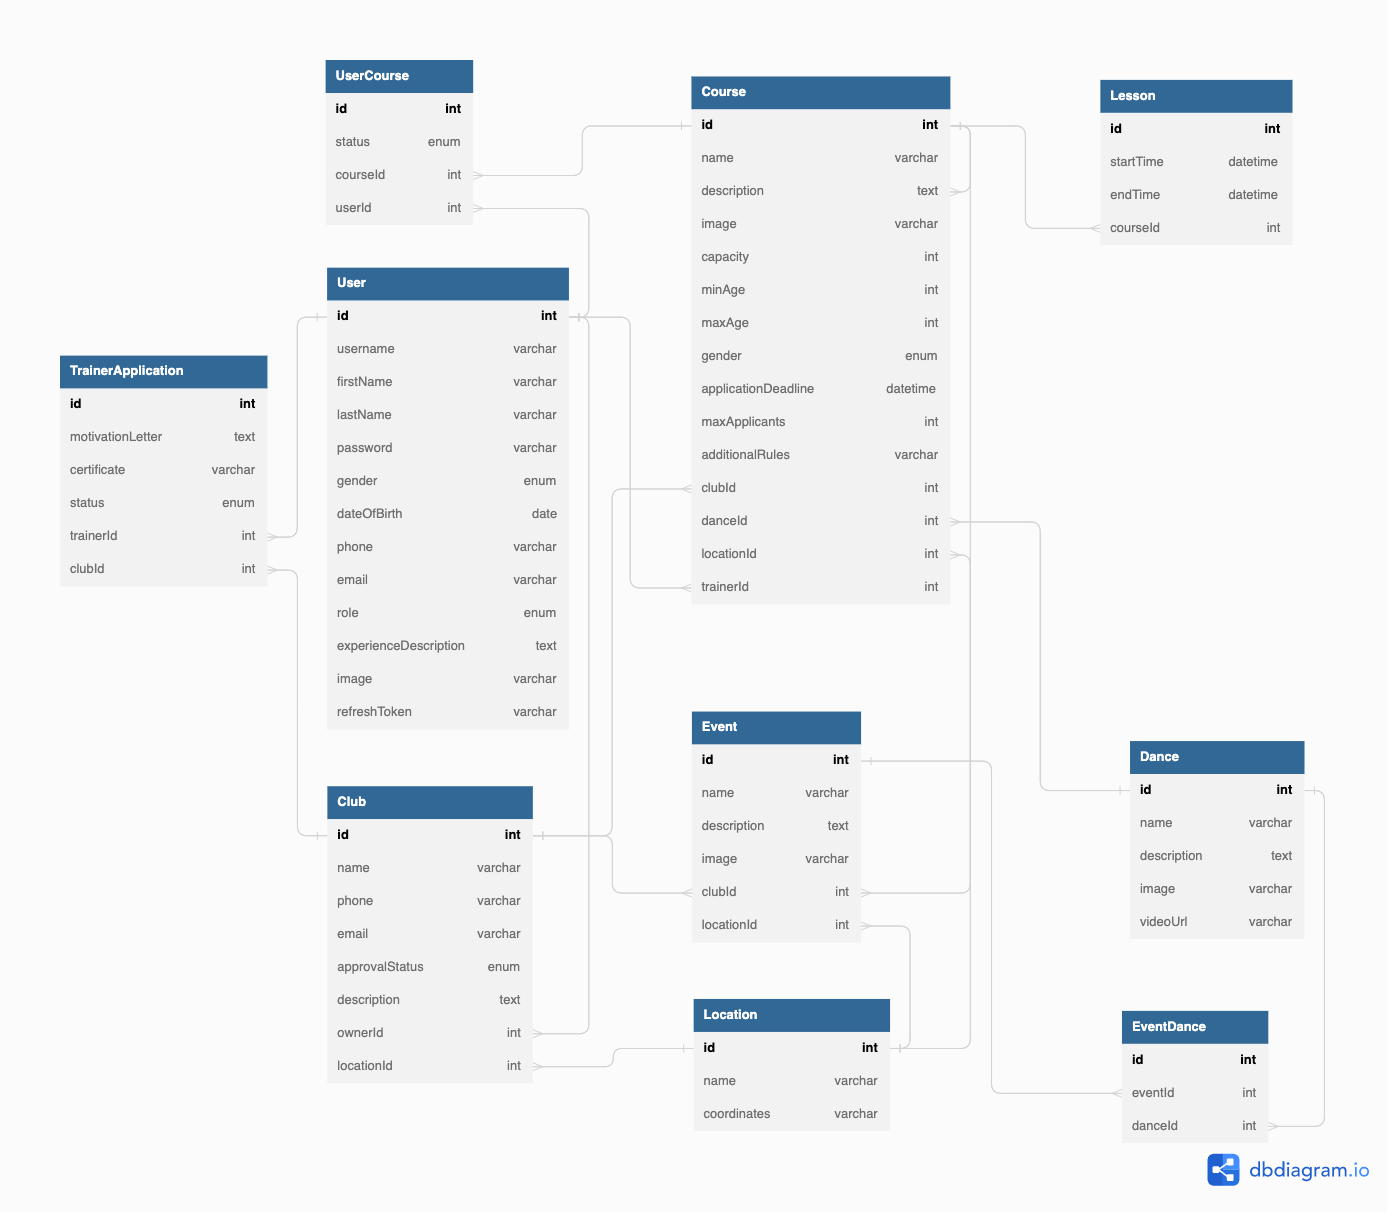
\includegraphics[scale=0.3]{slike/base_diagram.png}
			\centering
			\caption{Relacijski dijagram baze podataka.}
			\label{fig:promjen}
			\end{figure}
			
			\eject
			
			
		\section{Dijagram razreda}
		
			\noindent Na slikama su prikazani razredi koji pripadaju serverskoj strani aplikacije - konkretno modelima i 
			sučeljima koje oni nasljeđuju. Controlleri nisu definirani kao klase nego samo sadrže funkcije za upravljanje, stoga nisu 
			prikazani na klasnom dijagramu.
			Svi modeli nasljeđuju klasu Model. Model razredi preslikavaju strukturu baze podataka u aplikaciji
			Zbog lakše organizacije, dijagram je podijeljen u tri skupine, razredi su podijeljeni logički po dijelovima koji međusobno čine 
			logičku cjelinu ili nasljeđuju i implementiraju zajedničke enumeracuje ili sučelja.
			Iz naziva i tipova atributa u razredima moze se zaključiti vrsta ovisnosti među različitim razredima. \\

			\noindent Dijagram koji slijedi prikazuje modele User i Location te 
			model CourseModel.
			Model User implementira sučelje IUser, koje definira njegove atribute, i koristi enumeraciju Role i Gender. Role definira ulogu korisnika, a 
			Gender spol korisnika. Model Course implementira sučelje ICourse i korisni enumeraciju Gender za definiranje spola kojem je tečaj namijenjen, ako je za tečaj definirano ograničenje po spolu.
			\\
			\begin{figure}[H]
				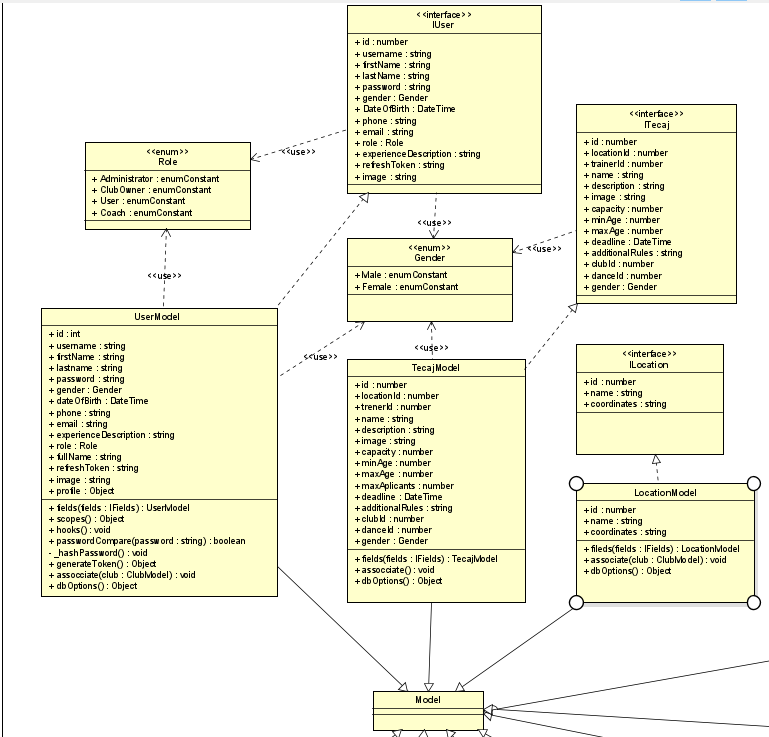
\includegraphics[scale=1.0]{slike/class1.png}
				\centering
				\caption{Dio klasnog dijagrama vezan uz modele User, Course i Location.}
				\label{fig:class1}
			\end{figure}		
			
			\noindent 
			Dijagram koji slijedi prikazuje modele Club, TrainerApplication i UserCourse.
			Model Club implemetnira sučelje IClub koji definira njegove atribute te korisni enumeraciju ApprovalStatus koja opisuje je li 
			administrator prihvatio tog kluba u sustavu ili ne. Klasa HttpError implementira sučelje IHttpError kojom lovimo moguće iznimke 
			nastale u kodu.
			\\
			\begin{figure}[H]
				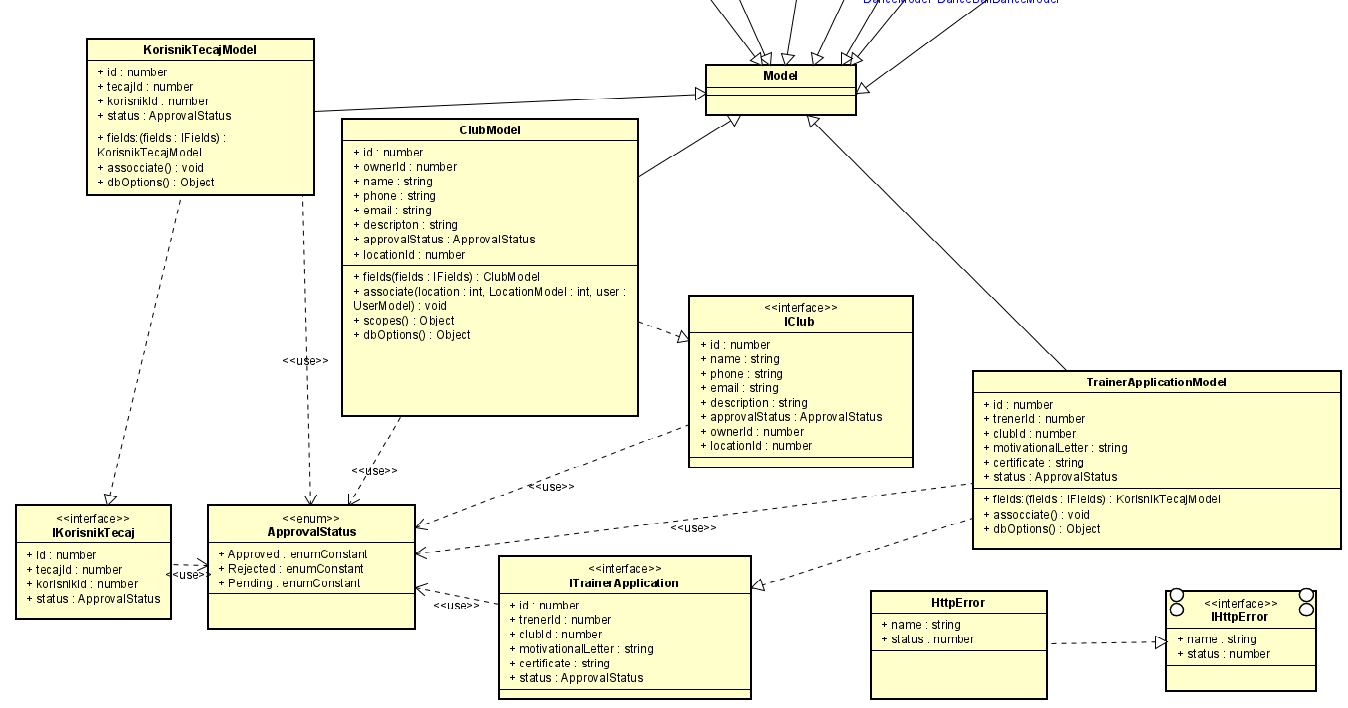
\includegraphics[scale=0.7]{slike/class2.png}
				\centering
				\caption{Dio klasnog dijagrama vezan uz modele Club, TrainerApplication i UserCourse.}
				\label{fig:class1}
			\end{figure}

			\noindent 
			Dijagram koji slijedi prikazuje modele Dance, Event, EventDance i Lesson. Svaki od modela implementira  svoje sučelje koje definira njegove atribute.
			\\
			\begin{figure}[H]
				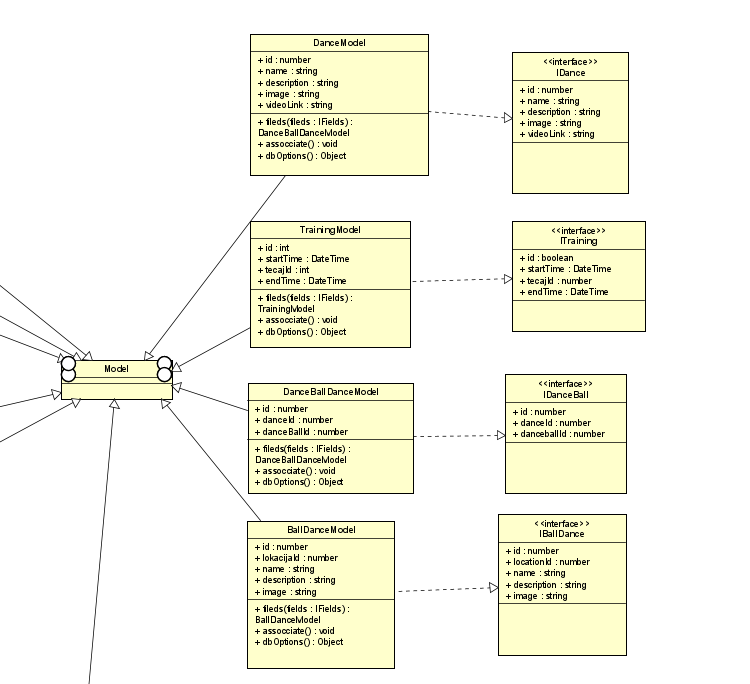
\includegraphics[scale=1.0]{slike/class3.png}
				\centering
				\caption{Dio klasnog dijagrama vezan uz modele Dance, Event, EventDance i Lesson.}
				\label{fig:class1}
			\end{figure}

		% 	\textit{Prilikom druge predaje projekta dijagram razreda i opisi moraju odgovarati stvarnom stanju implementacije}
			
			
			
		\eject
		
		\section{Dijagram stanja}
			
			
		% 	\textbf{\textit{dio 2. revizije}}\\
			
		% 	\textit{Potrebno je priložiti dijagram stanja i opisati ga. Dovoljan je jedan dijagram stanja koji prikazuje \textbf{značajan dio funkcionalnosti} sustava. Na primjer, stanja korisničkog sučelja i tijek korištenja neke ključne funkcionalnosti jesu značajan dio sustava, a registracija i prijava nisu. }
			
			
		% 	\eject 
		
		\section{Dijagram aktivnosti}

            \noindent Dijagram aktivnosti pokazuje proces prijave registriranog korisnika na tečaj. Prijavom u sustav njemu se prikazuje mapa sa listom tečajeva koji su slobodni za upis. Korištenjem filtera on može prilagoditi rezultate svojim preferencijama i pronaći tečaj koji njemu odgovara. Odabirom tečaja stranica ga odvodi na prikaz detalja istoga. Klikom na prijavu korisnik mora upisati tražene podatke i tada se njegova prijava šalje u bazu podataka, a stranica ga vraća na kartu sa prikazom svih tečaja. 

            \begin{figure}[H]
			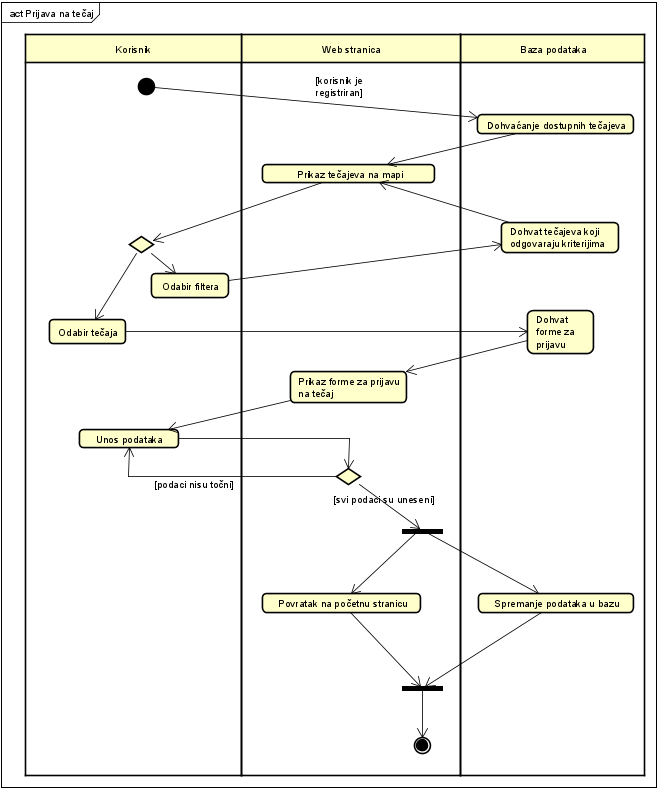
\includegraphics[scale=0.4]{slike/DijagramAktivnosti.PNG} %veličina slike u odnosu na originalnu datoteku i pozicija slike
			\centering
			\caption{Dijagram aktivnosti - prijava na tečaj}
			\label{fig:stanje}
		\end{figure}
		
		\section{Dijagram komponenti}
		
			\noindent Dijagram komponenti opisuje organizaciju i međuovisnost komponenti, interne strukture i odnose prema okolini. 
Postoje 3 Docker konteinera: jedan za bazu podataka ( port 3002), jedan za poslužiteljsku stranu (port 3001 ) i jedan za klijentsku stranu ( port 3000 ).
Klijentska strana podigne jedan html dokument i podigne virtualni DOM. View napravi virtualni DOM, provjerava podatke i pošalje na fizički DOM. View automatski puni fizički DOM s .json file-om. Nema slanja html dokumenta između klijentske i poslužiteljske strane. Klijentska strana preko http requestova traži od poslužiteljske strane informacije iz baze podataka. 
Postoji 10 „Controllera“ (za klub, tecaj, ples, dogadaj, dogadajPles, lekciju, lokaciju, trenerAplikaciju, korisnika i korisnikaTecaja) i njihovih 10 „Modela“.  Svaki entitet je model. Modeli su zadužni za dobavljanje podataka iz baze podataka. „Controller“  se nalazi na poslužiteljskoj strani i prima informaciju od „View“ komponente. On validira primljenu informaciju iz zahtjeva s klijentske strane, obavi sve što je potrebno za taj zadatak napraviti te vrati povratnu informaciju klijentu je li akcija uspješno obavljena. 
JavaScript „leaflet“ biblioteka služi za prikaz interaktivnih mapa
„Bycrpt“ je biblioteka koja služi za kriptiranje lozinke.

		
		\begin{figure}[H]
			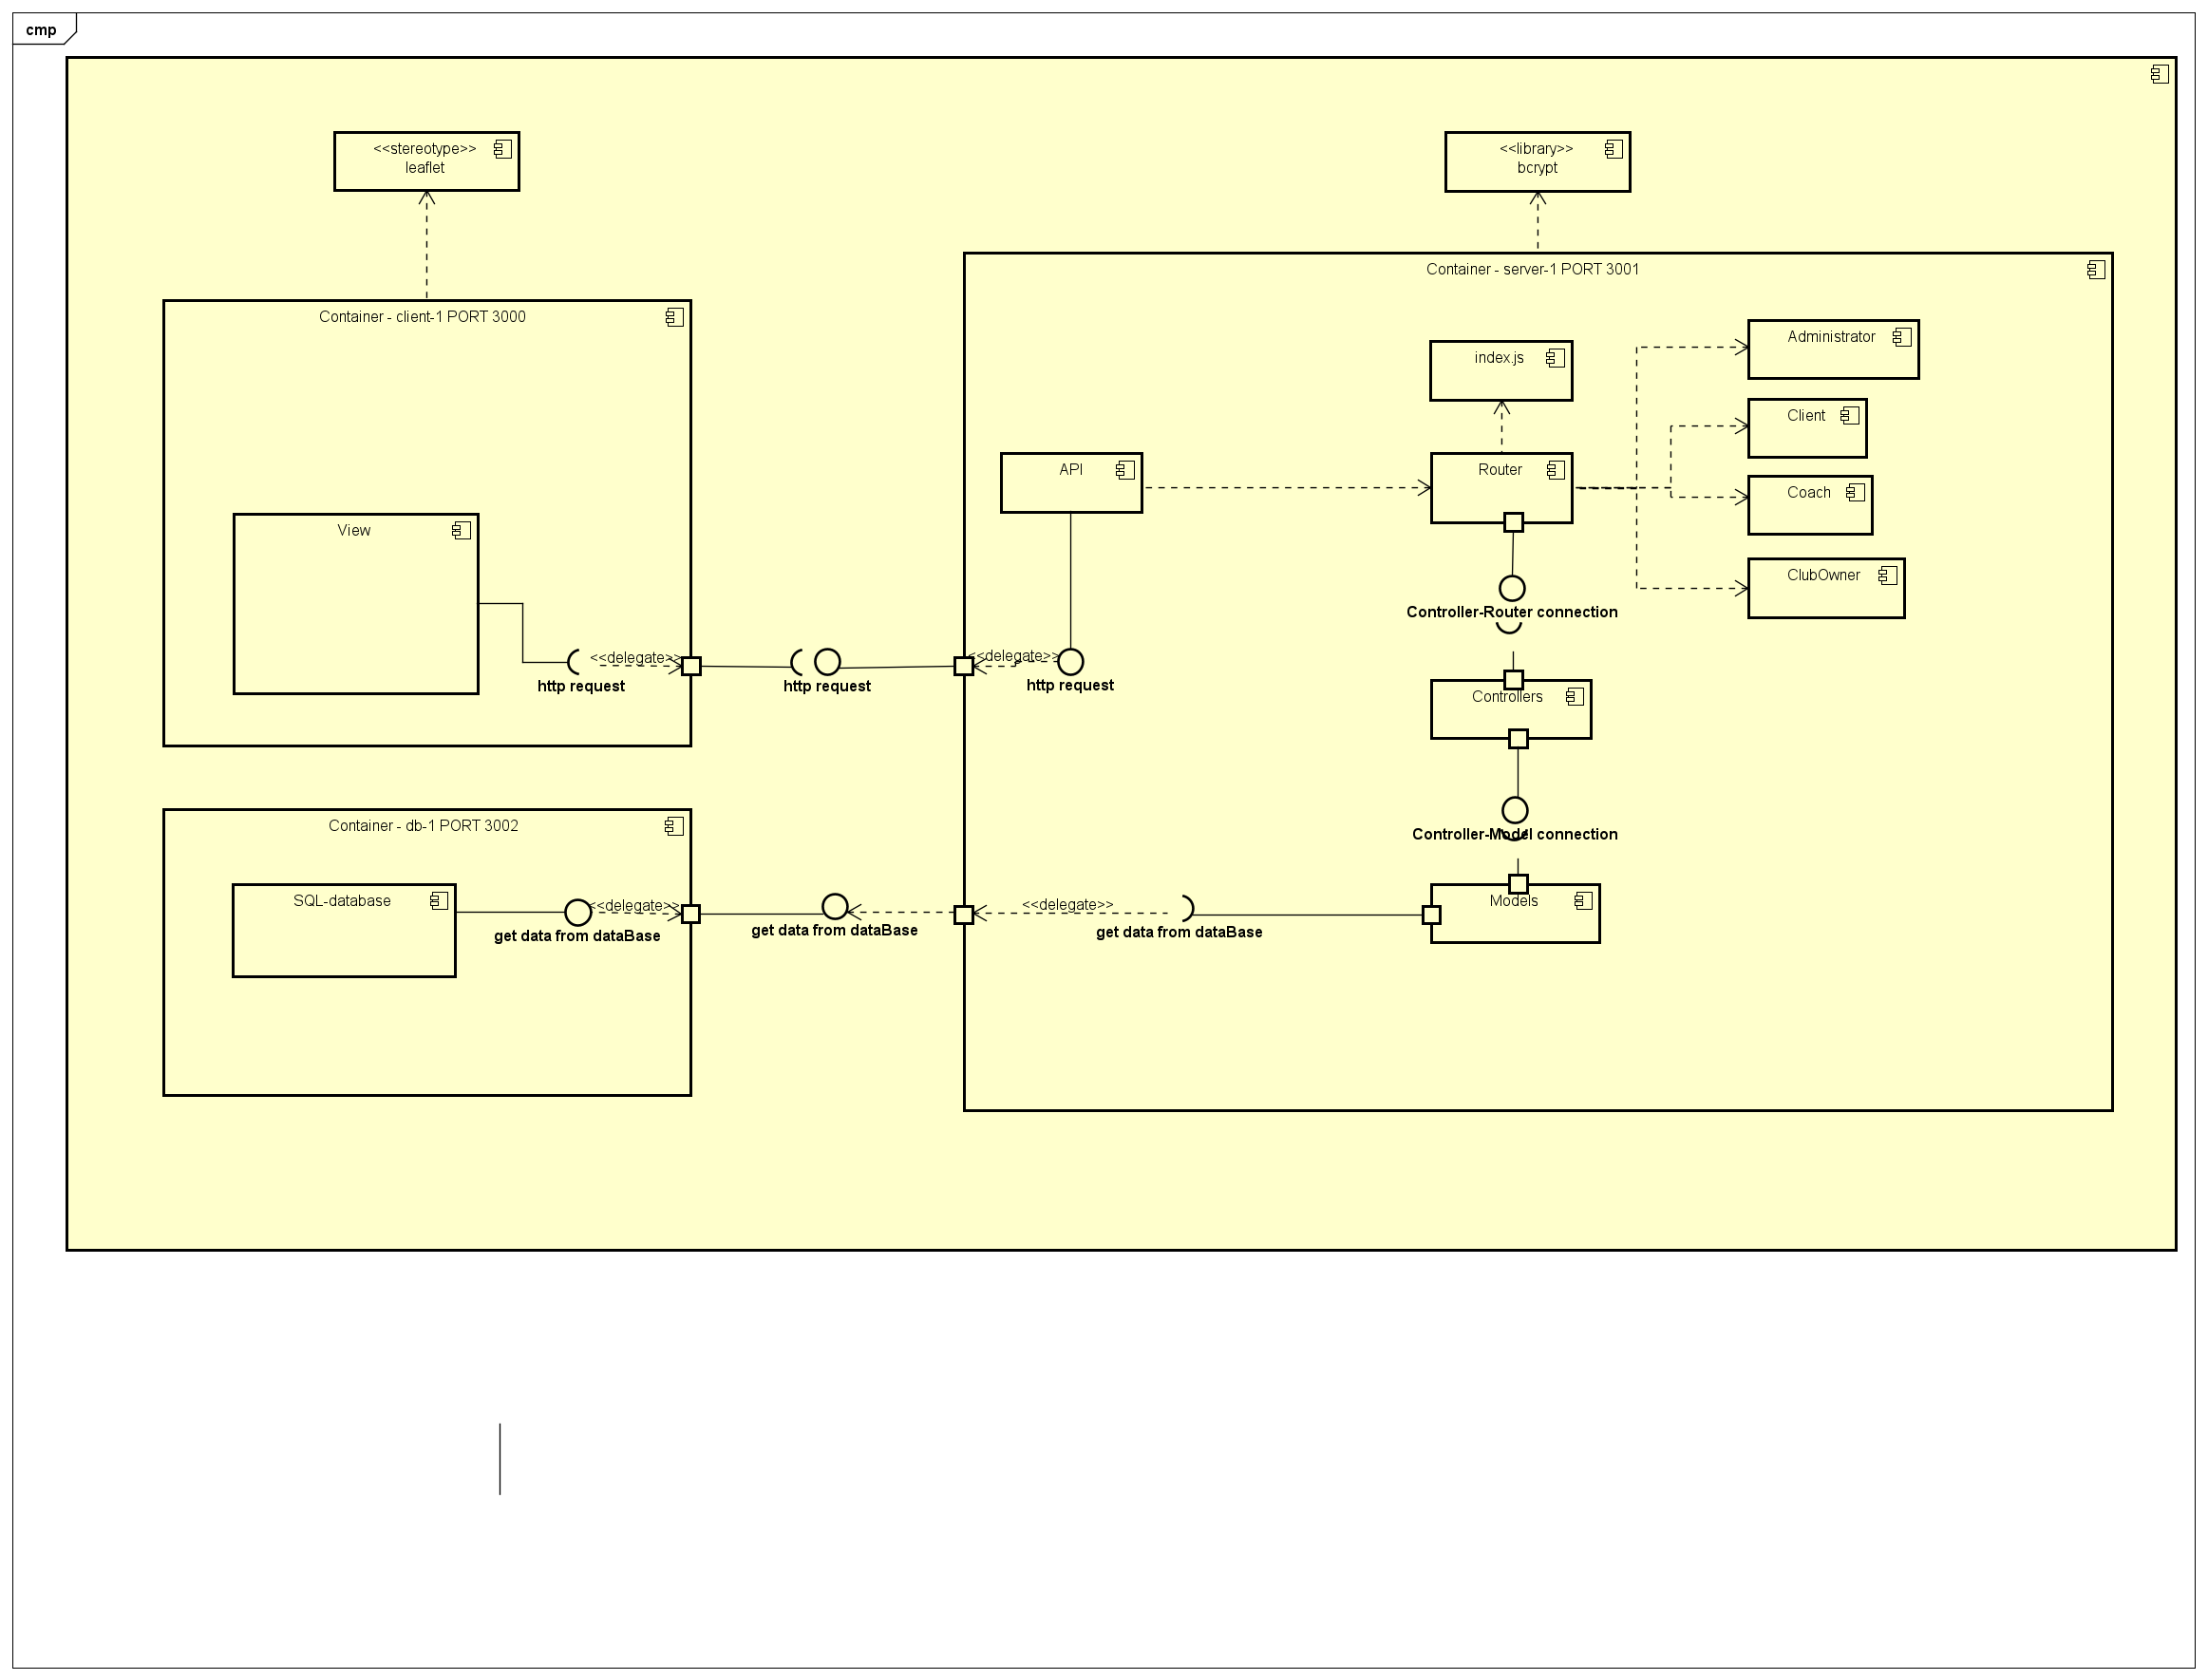
\includegraphics[scale=0.3]{slike/DijagramKomponenti.PNG} %veličina slike u odnosu na originalnu datoteku i pozicija slike
			\centering
			\caption{Dijagram komponenti}
			\label{fig:stanje}
		\end{figure}